\documentclass[onecolumn,abstract,paper=letter]{scrartcl}
% \usepackage[utf8]{inputenc}


% \usepackage[cmintegrals,cmbraces]{newtxmath}
% \usepackage{ebgaramond-maths}
\usepackage{mathpazo}
\usepackage{tgpagella}
\linespread{1.05}  
% \usepackage[onehalfspacing]{setspace}
% \usepackage[doublespacing]{setspace}
\usepackage[T1]{fontenc}

% \usepackage{baskervillef}
% \usepackage[varqu,varl,var0]{inconsolata}
% \usepackage[scale=.95,type1]{cabin}
% \usepackage[black,t1]{sourceserifpro}
% \usepackage[baskerville,vvarbb]{newtxmath}
% \usepackage[cal=boondoxo]{mathalfa}

\usepackage{mathtools}
\usepackage[usenames,dvipsnames]{xcolor}
\usepackage{tabu}
\usepackage{authblk}

\addtokomafont{disposition}{\rmfamily}
\addtokomafont{section}{\textsc}
\addtokomafont{caption}{\footnotesize}

% \RedeclareSectionCommand[style=section,indent=0pt]{part}
% \renewcommand*{\partformat}{\thepart\enskip}

\renewcommand{\thesection}{\Roman{section}} 
\renewcommand{\thesubsection}{\Alph{subsection}}
\renewcommand{\thesubsubsection}{\arabic{subsection}}

\usepackage{colortbl}
\definecolor{train}{RGB}{179,205,227}
\definecolor{val}{RGB}{254,217,166}
\newcommand{\train}{\cellcolor{train}Train}
\newcommand{\valdt}{\cellcolor{val}Validation}


%%%%%%%%%%%%%%%%%%%%%%%%%%%%%%%%%%%%%%%%%%%%%%%%%%
%%%%%   TITLE   %%%%%%%%%%%%%%%%%%%%%%%%%%%%%%%%%%
%%%%%%%%%%%%%%%%%%%%%%%%%%%%%%%%%%%%%%%%%%%%%%%%%%

\title{\textsc{\textmd{Cross-Validation Methodology \\ in Materials Science}}}
\author[1]{Julien Brenneck}
\author[2]{Alexander Dunn}
\author[2]{Anubhav Jain}
\affil[1]{University of Massachusetts Amherst}
\affil[2]{Lawrence Berkeley National Laboratory}
\date{SULI Summer 2018}

\renewcommand*{\Affilfont}{\normalsize\mdseries}
\renewcommand*{\Authfont}{\Large}
% \renewcommand*{\Authands}{, }


\newcommand{\etal}{\textit{et al}.\ }

\begin{document}

\maketitle


%%%%%%%%%%%%%%%%%%%%%%%%%%%%%%%%%%%%%%%%%%%%%%%%%%
%%%%%   ABSTRACT   %%%%%%%%%%%%%%%%%%%%%%%%%%%%%%%
%%%%%%%%%%%%%%%%%%%%%%%%%%%%%%%%%%%%%%%%%%%%%%%%%%

\begin{abstract}

High-throughput Materials Science has turned towards statistical and machine learning methods in the effort to rapidly accelerate material characterization and discovery.
While these methods promise to take advantage of the accumulating data, without effective quantification of performance and validation methodology there is no assurance that these models will generalize to new data.
% This is especially important in work that is largely comparing the performance of different models on materials data. 
This work highlights potential pitfalls and best practices in the cross-validation of these models.
In particular, it gives practical recommendations for cross-validation methodology.

% Material Science faces the insurmountable cost of experimentally collecting the properties of endless potential materials. 
% Computational techniques based on \textit{ab initio} simulation alleviate this burden, increasing the number of categorized materials by (?) orders of magnitude. 
% The computational cost of these techniques makes it still unfeasible to test all potential materials even in limited domains. 
% Models from statistics and machine learning are poised to utilize existing datasets to advance the search for new materials, as well as further the understanding of existing data.
% This paper attempts to highlight pitfalls and best practices in the use of these models. 


\end{abstract}

%%%%%%%%%%%%%%%%%%%%%%%%%%%%%%%%%%%%%%%%%%%%%%%%%%
%%%%%   INTRODUCTION   %%%%%%%%%%%%%%%%%%%%%%%%%%%
%%%%%%%%%%%%%%%%%%%%%%%%%%%%%%%%%%%%%%%%%%%%%%%%%%

\begin{section}{Introduction}
Materials Science faces the problem of experimentally collecting the properties of endless materials. 
Computational techniques based on \textit{ab initio} simulation alleviate this burden, increasing the ability to categorize materials by several orders of magnitude. 
The computational cost of these techniques makes it still unfeasible to test all potential materials even in limited domains, necessitating efficient higher level models of materials and their properties. 
Models from statistics and machine learning promise to utilize existing data sets to advance the search for new materials, as well as further the understanding of existing data.
This paper attempts to highlight pitfalls and best practices in the use of these models. 

A fundamental issue in the application of statistical and machine learning models is ensuring that the model learns to generalize.
A sufficiently powerful model may simply memorize local noise inherent to the training set without learning the overall trends in data, and hence would perform poorly on new data. 
While materials science has begun to adopt these models, there has been less adoption of rigorous validation methodology.
This work examines the main methods of validation in statistical and machine learning, the hold out test set and the cross-validation. 
While simple to implement, care must be taken in the application of these methods to avoid inadvertent and potentially invalidating bias in the results. 
The use of best practices, publishing of data, models, and hyper-parameters, and general reproducibility builds the confidence of a result. 

\subsection{Estimating Generalization Error}
The most common measure of the performance of a model is the test error, also known as generalization error.
This is the expected value of the loss function on model predictions of new data. Formally,
\begin{equation}
    \text{Err}_T = \mathbb{E} \left[ L(Y, \hat f(X)) \mid T  \right]
\end{equation}
where $\hat f$ is the trained predictor, $L$ is the loss function, $X$ and $Y$ represent the new test data, and $T$ is the fixed training set.
One can also define the expected test error
\begin{equation}
    \text{Err} = \mathbb{E} \left[ L(Y, \hat f(X)) \right] = \mathbb{E} \left[ \text{Err}_T \right]
\end{equation}
which takes the expectation of test error over the distribution of training sets $T$.
Training error is the average loss of the predictor over $T$, instead of a separate test set. 
In practice Err$_T$ is estimated using a single test set held out during training.

The loss functions considered in this paper are the Root Mean Squared Error (RMSE) and Mean Absolute Error (MAE) for regression, and Accuracy (the mean of 0-1 Loss) for classification.
Techniques in machine learning are highly dependant on the choice of loss function.
Intuitively, optimizing a model for one loss function will not necessarily cause the optimization of others, so a reasonable choice of loss function is critical and highly context dependant.

There are two main goals when training a model, \textit{Model Selection} and \textit{Model Assessment}.
The goal of model selection is comparison of several models and selecting the best model for the given data set. 
Model assessment estimates the generalization error of a single final model. 
When performing both model selection and then model assessment of the chosen model, the simplest method is splitting the data into test, validation, and training samples. 
The validation set is used to compare models during model selection, with the test set used in the final model assessment.
For smaller data sets, such as the ones in materials science, other methods such as Bayesian Information Critera (BIC) or re-sampling approaches such as the bootstrap and cross-validation are more appropriate.


\begin{subsection}{\textit{K}-Fold Cross-Validation}
The most common and generally applicable technique is cross-validation, particularly in the form of the $k$-fold cross-validation.
The data is split randomly into $k$ even, disjoint subsets. Each is then used as a validation set for a model trained on the remaining $k-1$ folds of data.
The mean of the $k$ computed validation errors is taken as the estimate of test error, though this effectiely estimates Err instead of Err$_T$, as noted by Hastie \etal \cite{hastie2009}.
The extreme case is \textit{leave one out cross-validation} (LOOCV) when $k=N$, and each validation set is a single sample point.
See \textit{Elements of Statistical Learning} \cite{hastie2009} or \textit{An Introduction to Statistical Learning} \cite{james2013} for further reference.

\begin{figure}[ht]
    \begin{center}
    \scriptsize
    \begin{tabu} to 0.65\textwidth{X[0.25,c]|X|X|X|X|X|X[0.1,c]}
    \tabucline{2-6}
    1 & \valdt & \train & \train & \train & \train & \\
    \tabucline{2-6}\noalign{\vskip 0.5em}\tabucline{2-6}
    2 & \train & \valdt & \train & \train & \train & \\
    \tabucline{2-6}\noalign{\vskip 0.5em}\tabucline{2-6}
    3 & \train & \train & \valdt & \train & \train & \\
    \tabucline{2-6}\noalign{\vskip 0.5em}\tabucline{2-6}
    4 & \train & \train & \train & \valdt & \train & \\
    \tabucline{2-6}\noalign{\vskip 0.5em}\tabucline{2-6}
    5 & \train & \train & \train & \train & \valdt & \\
    \tabucline{2-6}
    \end{tabu}
    \end{center}
    \caption{An example of 5-fold cross-validation. The data is randomly shuffled and then separated into 5 disjoint subsets of the same size, called folds. This gives 5 distinct train/validation splits.}
    \label{fig:folds}
\end{figure}

This method is not without trade-offs, and leaves the question of what value of $k$ should be used in practice. 
The current state of the theory around $k$-fold cross-validation \cite{arlot2010} is not yet conclusive, and can definitively state optimal choices of $k$ only in special cases.
Experimental results \cite{kohavi1995} and general best practice in the literature \cite{hastie2009} give $k=5$ or $k=10$ as reasonable values to use in general. 
While data sets can be found with almost any property, overarching trends recognized in the literature are that as $k$ increases, the variance of the cross-validation estimate increases and the bias goes to zero. For small values of $k$ there is a pessimistic bias, but low variance, and for the smallest values, $k < 5$, there is variance due to random sampling effects. 
There are cases when this does not hold, for example assuming a stability criteria \cite{arlot2010} such that models do not change under small perturbations of the data, LOOCV can have low variance and low bias.
For some classes of models, LOOCV is both stable and can be computed efficiently, making it a very practical methodology, but in a more general context it can have high variance and high computational time, making it a poor estimator and computationally unfeasible.
The computational burden of high $k$ values is of great practical importance, as the time complexity scales linearly in the number of folds, although it is highly amenable to parallelism. 
The choice of $k=5,10$ represents a choice that hopes to be safe in general, although it may sometimes not be optimal \cite{arlot2010}.


\end{subsection}

\begin{subsection}{Model Selection \& Nested Cross-Validation}

\end{subsection}

\begin{subsection}{Materials Data}

Scientists training models on data sets for materials science face several challenges.
One is the small size of experimental data, often less than 1000 samples. 
For predicting properties with complex relationships to the input features, there may not be enough data to build useful models. 
The universal technique for improving any problem in machine learning is adding more data, which is not always possible in experimental materials science. 
Simulation methods such as Density Functional Theory (DFT) alleviate this somewhat by allowing larger data sets to be computed, but the space of possible materials remains nearly infinite in comparison. 
This also has the problem that not all simulated materials can be synthesized, and that simulations are approximate and can introduce bias to the model. 

A second problem is the fact that problems in materials are often trying to extrapolate, instead of interpolate, from the data.
This is a fundamentally harder problem, and many current techniques are not equipped to solve it. 
For example, a scientist may try to predict a new semiconducting material, which would have to be unlike any existing material in their data. 
Models are fit around the existing data, and may fail to generalize at all outside the range of training samples.
Traditional validation methods may fail to account for this, as they largely measure how well a model interpolates. 

A third problem is that materials data can have a very large number of features in comparison to the number of data points.
The problem of representing materials data is non trivial, and is commonly done by encoding all existing and potentially useful numerical information about a material, for example compositional and structural data, in a vector format. 
This can lead to thousands of input features being created for data with only a few hundred samples. 
Feature selection is then commonly performed, but this can inadvertently introduce bias without preper methodology \cite{cawley2010}.
The high number of features can amplify this effect.  
This has been thoughouly examined in genomics \cite{ambroise2002}, where similar problems emerge. 


\end{subsection}



\end{section}

%%%%%%%%%%%%%%%%%%%%%%%%%%%%%%%%%%%%%%%%%%%%%%%%%%
%%%%%%%%%%%%%%%%%%%%%%%%%%%%%%%%%%%%%%%%%%%%%%%%%%

\begin{section}{Materials \& Methods}

The experiments in this study were run using scikit-learn (0.19.1) with Python (3.6.5) on NERSC jupyterhub computing resources. All jupyter notebooks to be available in supplementary materials. 
Additional data comes from Matminer (0.3.5).

\begin{subsection}{Experiment 1}
The classic example of over-fitting shows the divergence of test and training error as model complexity is increased. 
This highlights the bias-variance trade-off, a fundamental property in statistical learning.
A version of this is shown by Hastie \etal \cite{hastie2009}.
In this experiment a support vector machine (SVM) is fit to a regression data set that is normally distributed in the $x$ dimension, with $y = \sin(x) + \epsilon$, where $\epsilon$ is gaussian noise ($\sigma=0.1$). 
The SVM was fit with a Radial Basis Function (RBF) kernel and a regularization parameter of $C=1$.
We generate 100 distinct training and test sets from this distribution, then compare the test and training scores of the SVM model for various values of the hyper-parameter $\gamma$, which is a proxy for model complexity.
The range of $\gamma$ values used is $(10^{-4}, 10^{3})$.
\end{subsection}

\begin{subsection}{Experiment 2}
Highlighting the bias variance trade-off in the choice of $k$ for $k$-fold cross validation (CV) is difficult due to the fundamental inability to fully quantify CV variance, as there is no unbiased statistical estimator, and the bias can in practice be on the order of magnitude as the variance itself \cite{bengio2004}.
Despite this, it is possible to show the overall trends inherent to the choice of $k$, as the bias will decrease and variance will increase significantly as $k$ increases, even if the exact values are poor estimators of the true variance. 
Understanding the variance of CV is critical to understanding how the model will generalize, the ultimate goal of training such a model.
If the true model variance is high, we would expect there to be large changes in the model for small perturbations in the data, meaning the model has fit itself to noise.

This experiment computes the $k$-fold CV scores of a Support Vector Machine (SVM) using Radial Basis Function (RBF) kernel regression, for all possible values of $k$, that is $2$ to $N$ where $N$ is the number of samples.
The special case of $N=k$ is also called Leave One Out Cross Validation (LOOCV).
The CV error is estimated as the sample mean of all $k$ fold scores, and the standard deviation is estimated by the sample standard deviation of all $k$ fold scores.
The $D$ dimensional input data is generated from independent Normal distributions in each dimension.
The $1$ dimensional output data for regression is the product of the sine of each dimension, with gaussian noise added.
\begin{equation}
    Y_i = \prod_{j=1}^{D} \sin(X_{i,j}) + \epsilon
\end{equation}
\end{subsection}


\begin{subsection}{Experiment 3}
A more straightforward way of measuring variance relies on knowing the underlying distribution, or at the least having incredibly large amounts of data compared to its complexity. 
Instead of taking variance of the scores from each fold, the model can be trained on new data from the same underlying distribution multiple times, and the sample variance of CV estimates can be taken.
This more intuitively estimates the true model variance, but is computationally more expensive by at least one order of magnitude. 
This can be accomplished simply by repeating Experiment 1 multiple times with newly sampled data sets from the underlying distribution. 
This experiment did 10 repetitions, and took the mean and sample standard deviation of the 10 scores at every $k$ value.

\end{subsection}

% \begin{subsubsection}{Experiment ?}
% In the context of model selection, model variance can be measured through the variance of the model selected.
% In practice this means using CV to select a continuous hyper-parameter, and taking the sample variance of selected hyper-parameters.

% The same data and model is used as in the previous experiments.
% The selected hyper-parameter is $\gamma$.
% Raising the value of $\gamma$ effectively increases the complexity of the model, allowing it to capture more details of the data.
% A grid search on $(10^{-4}, 10^{4})$ is used with $K$-fold cross validation, with value of $K$ of $2,5,10,$ and $N$.
% For each value of $K$ a grid search is performed on a new data set sampled from the underlying distribution several times, and the sample variance of $\gamma$ values selected is taken.

% \end{subsubsection}

\begin{subsection}{Experiment 4}
To show how over-fitting during model selection can occur, a grid search hyper parameter optimization is performed on a selection of regression models.
Used in the final result are a Kernel Ridge Regression (KRR) with a polynomial basis function, a Gradient Boosted Tree Regression (GBTR), and a Gaussian Process Regression (GPR) with a Matern kernel.  
The elastic tensor data set from matminer is used, with the ElementProperty featurizer using the "magpie" default.
The highest cross-validation score (that of the selected model) is compared to training error, test set error, and nested cross validation error. 
The data is split into two equally size training and testing sets. 
The model selection is then performed using the training data with a 10-fold CV and a grid search, with the best selected model being retrained on the entire training set before test set evaluation. 
The training error is also evaluated using this retrained model.
The best score found during the cross-validation grid search is the CV score.
This is done separately for each class of models.
The nested cross-validation is done entirely on the training set, using a 5-fold CV within another 5-fold CV.
Over-fitting during model selection is not guaranteed to happen, and in this experiment it largely depends on the random train/test split. 
Random seeds were chosen to show how this type of over-fitting is a concern in practice, but it is not possible with this data to show that it always will happen. 



\end{subsection}




\end{section}

%%%%%%%%%%%%%%%%%%%%%%%%%%%%%%%%%%%%%%%%%%%%%%%%%%
%%%%%%%%%%%%%%%%%%%%%%%%%%%%%%%%%%%%%%%%%%%%%%%%%%

\begin{section}{Results}

\begin{subsection}{Experiment 1}
The result of this experiment matches the expected results shown in previous work \cite{hastie2009}.
As model complexity grows, training error is decreasing, but test error eventually begins to grow as the model over-fits the data.
See figure \ref{fig:train_test}.

\begin{figure}[ht]
    \centering
    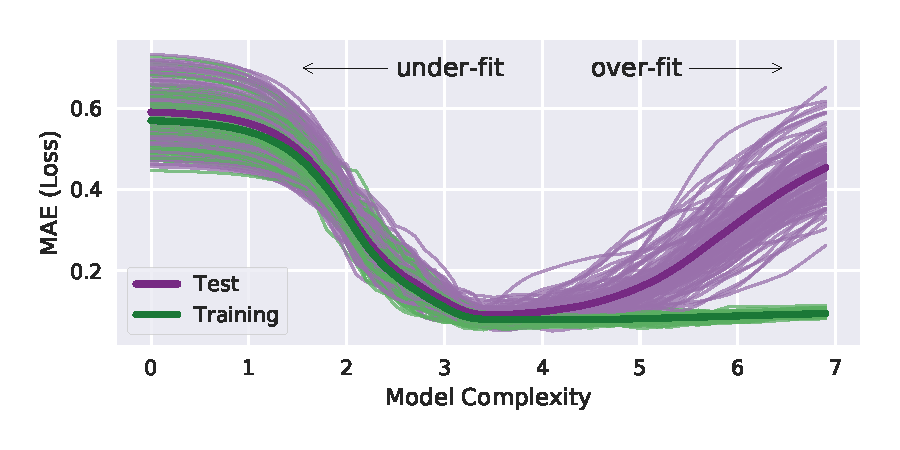
\includegraphics[width=0.75\textwidth]{plots/b-v+.pdf}
    \caption{As the model complexity increases, the training error is decreasing, but the test error grows once the model begins to over-fit.}
    \label{fig:train_test}
\end{figure}

\end{subsection}

\begin{subsection}{Experiment 2}

While the results of Bengio and Grandvalet \cite{bengio2004} show that this estimate is biased, with absolute numerical values that are likely not qualitatively meaningful, the experiment shows the general expected trends in variance.
The heavy pessimistic bias present for small $k$ values is apparent, as is the general trend of variance increasing with $k$. See figure \ref{fig:kfold-cv}

\begin{figure}[ht]
    \centering
    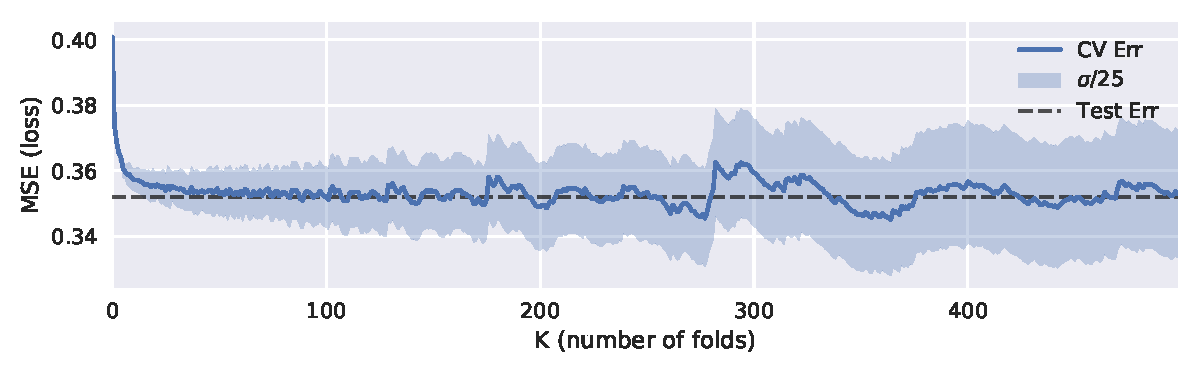
\includegraphics[width=\textwidth]{plots/kfold-cv-std-8x3.pdf}
    \caption{Effects of varying $K$ in $K$-Fold cross-validation.}
    \label{fig:kfold-cv}
\end{figure}
\end{subsection}

\begin{subsection}{Experiment 3}
This experiment shows the same general trends of variance increasing with $k$ and high bias for small $k$ as the previous experiment. 
One effect that is apparent here, and not visible in experiment 2, is the variance for low $k$, likely caused by sampling variance inherent to the small number of folds.
\begin{figure}[ht]
    \centering
    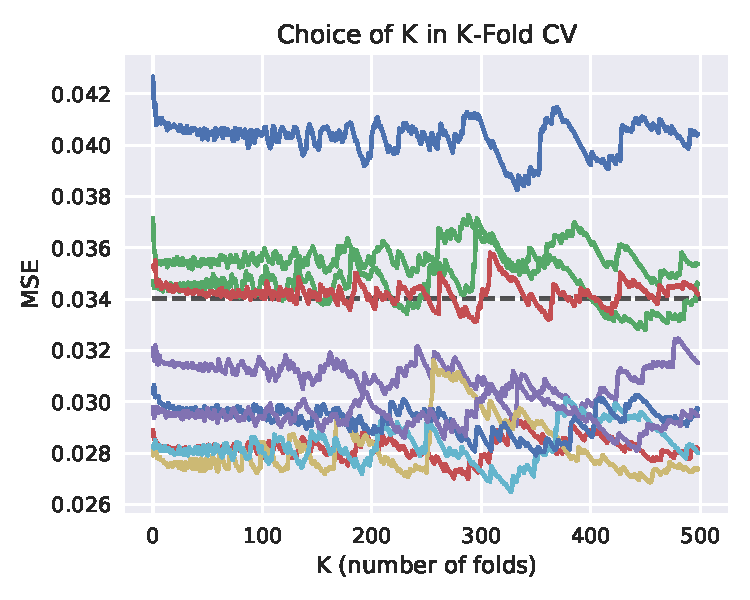
\includegraphics[width=0.32\textwidth]{plots/kfold-alt-all-5x4.pdf}
    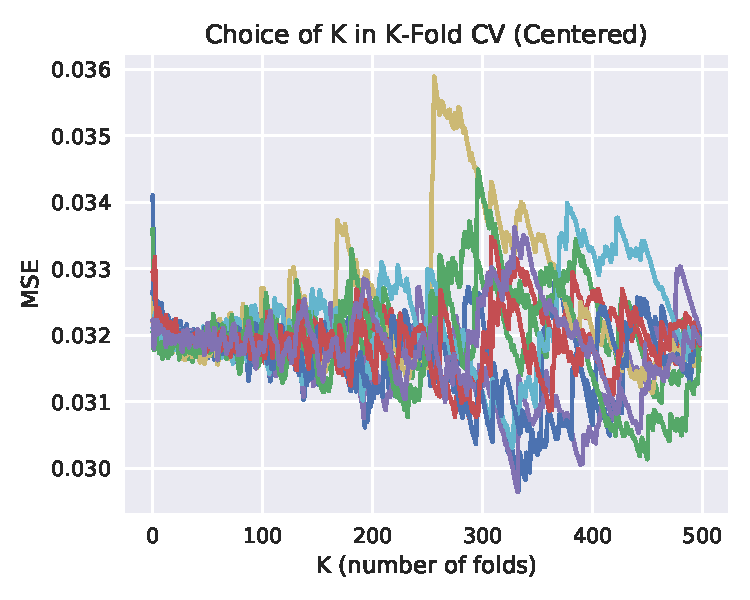
\includegraphics[width=0.32\textwidth]{plots/kfold-alt-center-5x4.pdf}
    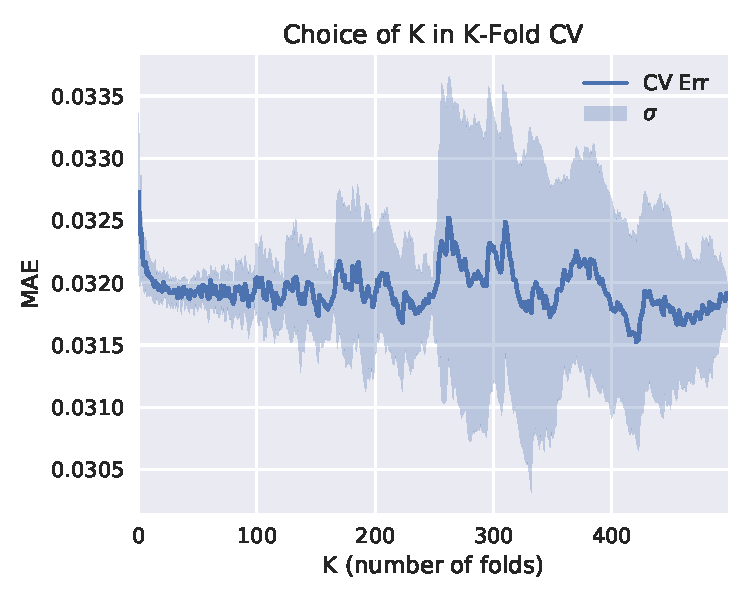
\includegraphics[width=0.32\textwidth]{plots/kfold-alt-5x4.pdf}
    \caption{After removing data set bias due to random sampling from the underlying distribution, a trend in the variance appears.}
    \label{fig:kfold_cv_alt}
\end{figure}

Simply taking the sample mean and variance at each $K$ gives a strange result.
The bias is as expected, but the variance is nearly constant.
This variance is due to the bias inherent to each training set.
If we plot the CV estimate curves individually (shown below) we see that the variance due to this bias is causing the effect.
If the bias is removed from the results (centering them using the low bias/variance region between $K=(25,75)$) we get the expected growth in variance as $K$ is increased. 
Note that one standard deviation here is an order of magnitude smaller than in the previous test, so clearly the exact numbers from CV fold variance (the only method usable in practice) are likely too heavily biased to give meaningful estimates. For example the fold std is 0.33 at $K=400$, data set std is 0.004 at $K=400$.
This method of re-centering the data is largely ad hoc, but highlights some of the difficulties in measuring cross-validation variance. 
\end{subsection}

\begin{subsection}{Experiment 4}
This experiment successfully shows how it is possible to over-fit during model selection. 
The over-fit cross-validation error seriously underestimates the true test error. 
We see that nested cross-validation alleviates this somewhat.
As in the first experiment, the training error is a heavily biased estimator for generalization error. 

\begin{table}[ht]
  \begin{minipage}[b]{0.69\textwidth}
    \centering
    \small
    \taburulecolor{gray}{
    \tabulinesep=0.5em
    % \vspace{-3em}
    \begin{tabu} to \textwidth{X[4] X[4,r] X[4,r] X[4,r] X[4,r]}
    \tabucline{-}
    Model  & Train Err & 10-fold CV Err & Nested CV Err & Test Err \\
    \tabucline{-}
    KRR  & \textcolor{BrickRed}{\bfseries 10.17} & \textcolor{BurntOrange}{\bfseries 18.26} & \textcolor{NavyBlue!75!gray}{\bfseries 21.41} &  \textcolor{ForestGreen}{\bfseries 21.61}   \\
    GBTR & \textcolor{BrickRed}{\bfseries  3.37} & \textcolor{BurntOrange}{\bfseries 14.37} & \textcolor{NavyBlue!75!gray}{\bfseries 16.38} & \textcolor{ForestGreen}{\bfseries 20.90}   \\
    GPR  & \textcolor{BrickRed}{\bfseries  0.00} & \textcolor{BurntOrange}{\bfseries 32.63} & \textcolor{NavyBlue!75!gray}{\bfseries 33.96} & \textcolor{ForestGreen}{\bfseries 35.45}   \\
    \tabucline{-}
    \end{tabu}
    \vspace{2.25em}
    }
    \end{minipage}
  \begin{minipage}[b]{0.3\textwidth}
    \centering
    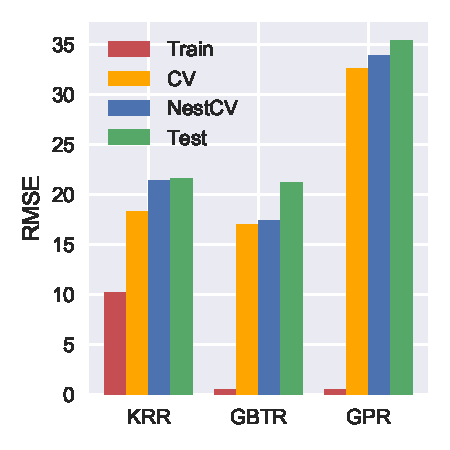
\includegraphics[width=0.98\textwidth]{plots/errors-3x3.pdf}
  \end{minipage}
    \label{tbl:overfit}
    \caption{Comparing prediction errors of an over-fit model on bulk modulus data. Model selection CV estimates can seriously underestimate true test error.}
\end{table}



\end{subsection}



\end{section}

%%%%%%%%%%%%%%%%%%%%%%%%%%%%%%%%%%%%%%%%%%%%%%%%%%
%%%%%%%%%%%%%%%%%%%%%%%%%%%%%%%%%%%%%%%%%%%%%%%%%%


%%%%%%%%%%%%%%%%%%%%%%%%%%%%%%%%%%%%%%%%%%%%%%%%%%
%%%%%%%%%%%%%%%%%%%%%%%%%%%%%%%%%%%%%%%%%%%%%%%%%%


%%%%%%%%%%%%%%%%%%%%%%%%%%%%%%%%%%%%%%%%%%%%%%%%%%
%%%%%%%%%%%%%%%%%%%%%%%%%%%%%%%%%%%%%%%%%%%%%%%%%%

% \begin{section}{Discussion}

% \subsection{Model Selection and Evaluation}
% The process of model selection, choosing a model and hyper-parameters, can heavily bias estimated model performance without proper methodology. 
% A pitfall in materials is in feature selection, which needs to be considered as part of model selection.
% The large number of features in materials data can increase this bias. 
% Feature selection needs to be considered an integral part of model selection \cite{cawley2010}.


% \end{section}

%%%%%%%%%%%%%%%%%%%%%%%%%%%%%%%%%%%%%%%%%%%%%%%%%%
%%%%%%%%%%%%%%%%%%%%%%%%%%%%%%%%%%%%%%%%%%%%%%%%%%

\begin{section}{Conclusion}


\begin{itemize}
    \item Use a hold out test set for model selection.
    \item Consider nested CV or Bayesian methodology for small data.
    \item Over-fitting in model selection is a problem in practice, and can cause over or under fitting in the final model.
    \item Feature selection can cause bias if not part of cross-validation.
\end{itemize}

\begin{itemize}
    \item Use a validation set or $k$-fold CV with $k=5$ or $k=10$ depending on size of data, and avoid LOOCV (in general).
    \item Use repeated k-fold CV to increase confidence in CV estimate.
    \item Model selection and feature selection need to be internal to validation scheme to avoid over-fitting.
    \item A good methodology is using a test / train split, then using CV for model selection on the training data, and measuring final model performance on the test data.
\end{itemize}



\end{section}

%%%%%%%%%%%%%%%%%%%%%%%%%%%%%%%%%%%%%%%%%%%%%%%%%%
%%%%%%%%%%%%%%%%%%%%%%%%%%%%%%%%%%%%%%%%%%%%%%%%%%

\subsection*{Acknowledgements}
{\small 
This work was supported in part by the U.S. Department of Energy, Office of Science, Office of Workforce Development for Teachers and Scientists (WDTS) under the Science Undergraduate Laboratory Internship (SULI) program.
Additional funding was provided by the U.S. Department of Energy, Office of Basic Energy Sciences, Early Career Research Program.
}

\scriptsize
\nocite{*}
\bibliography{MLMS}
\bibliographystyle{plain}

\end{document}